\section{Bug}
\label{sec:Bug}

This is an 'umbrella' term.

Usually a \index{Bug}\emph{Bug} is a flaw in a component (or system) that can cause the component (or system) to fail to perform its required function, e.g. an incorrect statement or data definition.

But not every Bug is a \index{Defect}Defect [p.\pageref{sec:Defect}]. You cannot always be sure, what is the root cause of a flaw. An \emph{Error} (a human mistake) in programming code can lead to a \emph{Defect}. Sometimes a Bug can be nothing than a \emph{Failure}\footnote{~Deviation of the component or system from its expected delivery, service or result.}, or a \emph{Mistake}, or an \emph{Error}\ldots 

It will be more convenient, if we will use a common term for all this artifacts~\textemdash~the \emph{Bug}.

ANY deviation from the expected result during testing can be treated as a \emph{Bug}. 

But not every deviation is a bug.

\begin{quote}
Women wear dresses and earrings (this is an expectation). 

When you will see a women wearing trousers, then '\textit{Whoa, the actual result differs from the expected, this is a bug!}'? 

Clearly not.
\end{quote} 

\subsection{Why it is called 'A Bug'}

A typical version of the story of the 'bug' term is:

\begin{quote}
In September 9, 1945, \index{Grace Hopper}Grace Hopper\footnote{~Grace Brews Murray Hopper (December 9, 1906 – January 1, 1992), the future United States Navy Rear Admiral; one of the first programmers of the Harvard Mark I computer in 1944; invented the first compiler for a computer programming language; one of those who popularized the idea of machine-independent programming languages which led to the development of COBOL, one of the first high-level programming languages.} work on the 'Mark II' computer at the Harvard Faculty.

Operators traced an error in the 'Mark II' to a moth trapped in a relay. 

Dead bug was carefully removed and taped to the log book. 

Stemming from the first bug, today we call errors or glitches in a program a bug.

Amen.
\end{quote} 

\begin{figure}[!h]
\centering
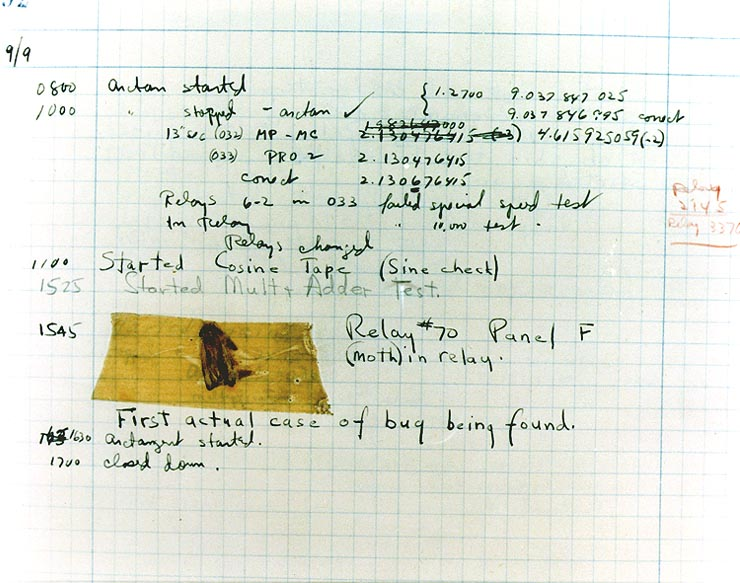
\includegraphics[width=0.8\linewidth]{debugging}
\caption{\ttfamily{'First actual case of bug being found'. September 9, 1947}}
\label{fig:Debugging}
\end{figure}

Well\ldots 

You can call me a naïve idiot, but what if into the 'Mark II' has been climbed and deadly shocked not a moth, but a cat?

\begin{quote}
Or a programmer?
\end{quote}

In fact, the term "bug" to describe defects already has been a part of engineering jargon for many decades and predates computers and computer software. It may have originally been used in hardware engineering to describe mechanical malfunctions. 

For instance, \index{Thomas Edison}Thomas Edison wrote the following words in a letter to an associate in 1878\footnote{~Edison to Puskas, 13 November 1878, Edison papers, Edison National Laboratory, U.S. National Park Service, West Orange, N.J., cited in Hughes, Thomas Parke (1989). American Genesis: A Century of Invention and Technological Enthusiasm, 1870-1970. Penguin Books. p. 75. ISBN 978-0-14-009741-2.}:

\begin{quote}
    It has been just so in all of my inventions. The first step is an intuition, and comes with a burst, then difficulties arise~\textemdash~this thing gives out and [it is] then that "Bugs"~\textemdash~as such little faults and difficulties are called~\textemdash~show themselves and months of intense watching, study and labor are requisite before commercial success or failure is certainly reached.
\end{quote} 

In '40 every computer guy was a radio mechanic or somehow similar to it (you cannot operate an old fashioned computer without being able to repair it several times by a day by your own hands and an soldering iron). So, computer operators were already familiar with the engineering term 'bug'. They amusedly kept the insect in the computer log, because it is really fun to discover a personalization of 'a bug'. That's why they noted it as the "\textit{First actual case of bug being found}" :)

\begin{quote}
Today this log book, complete with attached moth, is part of the collection of the Smithsonian National Museum of American History.

Why a log: on those days every interaction with the computer had to be noted on a paper.                                                                                        \end{quote} 

And Grace Hopper did not find the bug, as she readily acknowledged that. The notation "\textit{First actual case of bug being found}" was made by a group of computer operators, including William "Bill" Burke~\textemdash~maybe he wrote the famous sentence.

And the date in the log book was September 9, 1947, not 1945. The related term "debug" also appears to predate its usage in computing: the Oxford English Dictionary's etymology of the word contains an attestation from 1945, in the context of aircraft engines.
